\chapter{Обзор подходов к компиляции гетерогенных приложений}\label{ch:overview}

\section{Логическое и физическое представление гетерогенных систем}\label{sec:overview/logical}

\subsection{Логическая модель памяти для GPGPU}\label{subsec:overview/logical/memory}

При работе с графическими API для вычислений (такими как OpenCL, SYCL, Cuda и прочие), программисту приходится иметь дело с несколькими уровнями памяти.
Базовое разделение это \textbf{память хоста} -- память хостовой машины, обычно это что-то вроде обычной RAM и \textbf{память устройства}, устроенная гораздо сложнее.

В обычном случае память устройства бывает следующих видов:

\begin{itemize}
\item \textbf{Глобальная} -- память на устройстве обычно большого объёма и доступная каждому EU.
\item \textbf{Виртуальная разделяемая} -- участки памяти непосредственно отображаемые на память хоста.
\item \textbf{Константная} -- память, изменение которой в программах выполняемых на устройстве запрещено.
\item \textbf{Локальная} -- память доступная только потокам внутри рабочей группы.
\item \textbf{Приватная} -- память (обычно очень небольшое её количество) доступная только конкретному EU.
\end{itemize}

Здесь бывают тонкости и нюансы в терминологии. Например память, которая в SYCL называется приватной, в CUDA называется локальной, локальная называется разделяемой, а разделяемая глобальная называется унифицированной. Но с точностью до переименований все современные программные интерфейсы работают более-менее с одной логической моделью. Далее в этой работе будет использоваться терминология SYCL.

Обычно тип памяти напрямую запрашивается при работе с программным интерфейсом как на листинге~\cref{lst:oclapi}. Такие вызовы с хоста по сути являются обращениями к графическому рантайму или как его иначе называют UMD (user-mode driver). Он обрабатывает такого рода запросы и комбинируя их в пакеты отправляет их к нижележащему интерфейсу операционной системы.

\nomenclature{\(UMD\)}{user-mode driver, обычное название графического рантайма}
\nomenclature{\(KMD\)}{kernel-mode driver, драйвер операционной системы, требующий привилегированного исполнения}

\begin{ListingEnv}[!h]
    \captiondelim{ } 
    \caption{Пример запроса глобального буффера в OpenCL API}\label{lst:oclapi}
    \begin{lstlisting}[language={[ISO]C++}]
  cl_context Context;
  cl_mem Buf;
  cl_int Err;
  Context = clCreateContextFromType(NULL, CL_DEVICE_TYPE_GPU, NULL, 
                                    NULL, &Err);
  // .....
  Buf = clCreateBuffer(Context, CL_MEM_READ_WRITE, BUFSZ * sizeof(int), 
                       NULL, &Err);
    \end{lstlisting}
\end{ListingEnv}

Мы будем называть такого рода вызовы API-вызовами (API call). Многие современные программные интерфейсы такие как SYCL и CUDA делают эти вызовы неявными. Другие, такие как OpenCL, наоборот, стараются делать явные вызовы. В хорошо спроектированной программе количество такого рода вызовов надо минимизировать так как такого рода общение с рантаймом не бесплатно и при неправильном использовании вносит ненужные расходы времени и памяти.

В данном случае API-вызов \lstinline!clCreateBuffer! запрашивает создание буфера в глобальной памяти. В некоторых случаях компилятор может оптимизировать работу с памятью, например сделав stateless to stateful преобразование и тогда этот буфер окажется в несколько другой памяти (при соблюдении ряда условий). Но программист всегда оперирует с логической моделью, так как это единственный способ написать общий код для нескольких устройств гибридной системы.

\begin{figure}[ht]
    \centerfloat{
        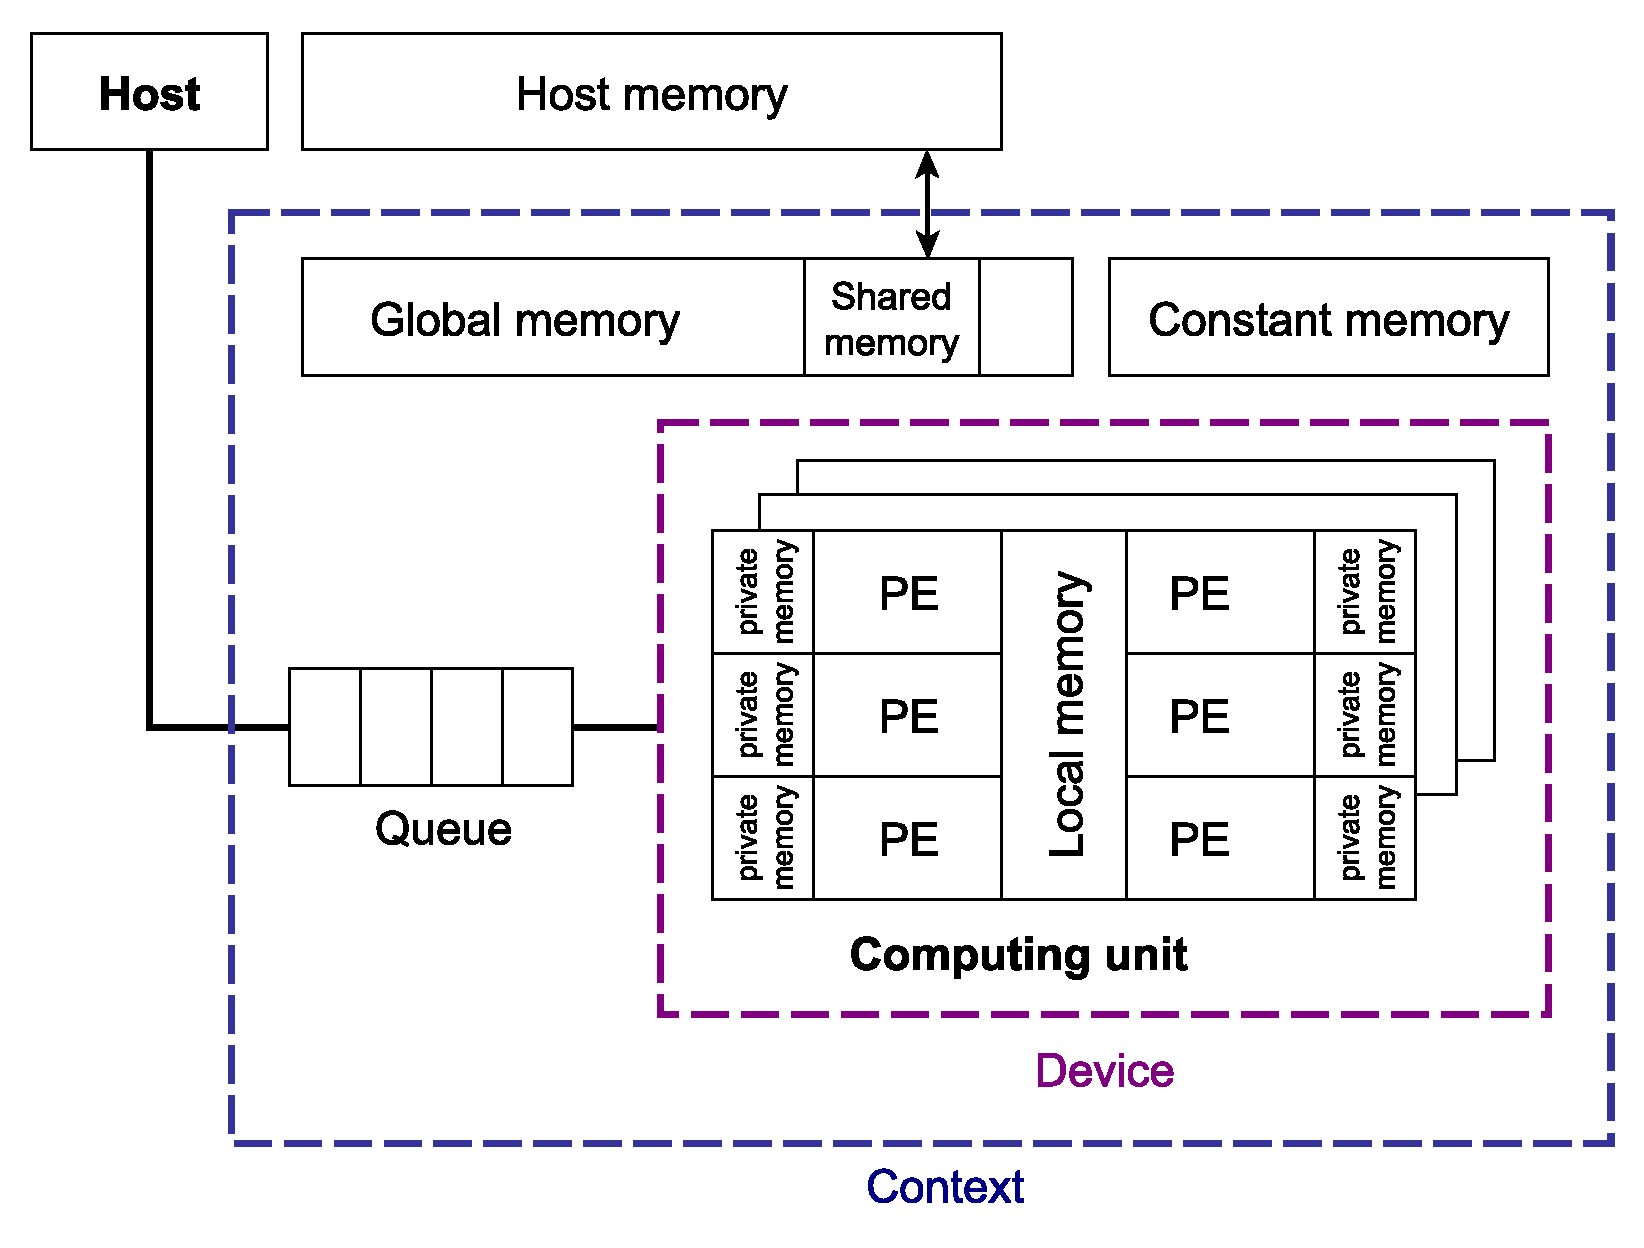
\includegraphics[scale=0.6]{Vladimirov/images/logical-memory.pdf}
    }
    \caption{Логическая модель памяти}\label{fig:logical-memory}
\end{figure}

Логическая модель памяти, характерная для таких API, как OpenCL и SYCL, представлена на рисунке~\cref{fig:logical-memory}. Ключевым понятием является computing unit (CU), комбинирующий несколько исполнительных устройств. Каждый computing unit это элемент кооперативной многозадачности внутри GPU. Все исполнительные устройства в пределах CU обладают доступом к общему пространству -- локальной памяти. Это небольшая и быстрая общая память. Она очень важна в таком виде. Но ещё важнее, что итерационное пространство рабочей группы позволяет потокам в её пределах ждать друг друга на семафорах, называемых часто барьерами.

Чтобы проиллюстрировать концепцию барьера, допустим у нас есть гнездо циклов с внутренним параллелизмом, представленное на листинге~\cref{lst:nobarrier}.

\begin{ListingEnv}[!h]
    \captiondelim{ } 
    \caption{Гнездо циклов с внутренним параллелизмом}\label{lst:nobarrier}
    \begin{lstlisting}[language={[ISO]C++}]
for (auto i : Ni)
  for (auto j : Nj)
    parallel for (auto k : Nk)
      do(i, j, k);
    \end{lstlisting}
\end{ListingEnv}

Это довольно плохой случай, так как мы можем распараллелить только самый вложенный цикл и получается, что мы должны постоянно входить в параллельное исполнение и выходить из него. Но если порядок по $k$ не важен, и $N_k$ не велико, то мы можем воспользоваться барьерами рабочей группы. Тогда это гнездо циклов трансформируется в следующий более выгодный вид, приведённый на листинге~\cref{lst:localbarrier}.

\begin{ListingEnv}[!h]
    \captiondelim{ } 
    \caption{Гнездо циклов с барьером внутри}\label{lst:localbarrier}
    \begin{lstlisting}[language={[ISO]C++}]
parallel for (auto k : Nk)
  for (auto i : Ni)
    for (auto j : Nj) {
       do(i, j, k);
       barrier(k);
    }
    \end{lstlisting}
\end{ListingEnv}

Разница в том что теперь для каждого элемента параллелизма оба дорогих вложенных цикла исполняются на своём исполнительном устройстве. Эта техника на некоторых бенчамрках, таких как перемножение матриц или битоническая сортировка позволяют выиграть до тридцати процентов производительности и более даже в простом скалярном случае.

Чтобы сделать пример более реалистичным, рассмотрим типичное гнездо циклов для практически важной задачи перемножения матриц, приведенное на листинге~\cref{lst:gemmnested}. Матрицы разбиты на тайлы и для каждого тайла мы в первом цикле запускаем копирование в локальную память и вычисление небольшого произведения в локальной памяти (мы должны помнить что она не велика). Во втором цикле мы собираем результаты обратно в глобальную память.

\begin{ListingEnv}[!h]
    \captiondelim{ } 
    \caption{Матричное перемножение с локальной памятью и вложенным параллелизмом}\label{lst:gemmnested}
    \begin{lstlisting}[language={[ISO]C++}]
private S = 0;
for (Tile = 0; Tile < NumTiles; ++Tile) {
  parallel for(auto Wi: Workitems)
    copy_global_to_local(Tile, Wi); 
  parallel for(auto Wi: Workitems)
    S = calculate_local_mmult(wi);
}
parallel for(auto Wi: Workitems)
  update_global_memory(S, Wi); 
    \end{lstlisting}
\end{ListingEnv}

Очевидно здесь внешний цикл никак не распараллелен и это приводит к существенным накладным расходам. Чтобы этого избежать, давайте формально введём барьеры и инвертируем циклы точно по той же схеме, которую мы использовали на листинге~\cref{lst:localbarrier}.

\begin{ListingEnv}[!h]
    \captiondelim{ } 
    \caption{Матричное перемножение с барьерами}\label{lst:gemmbarrier}
    \begin{lstlisting}[language={[ISO]C++}]
parallel for(auto Wi: Workitems)
  for (Tile = 0; Tile < NumTiles; ++Tile) {
    copy_global_to_local(Tile, Wi);
    barrier;
  }
parallel for(auto Wi: Workitems)
  for (Tile = 0; Tile < NumTiles; ++Tile) {
    S = calculate_local_mmult(wi);
    barrier;
  }
    \end{lstlisting}
\end{ListingEnv}

Результат такого рода инверсии приведён на листинге~\cref{lst:gemmbarrier}. Теперь мы имеем два паралелльных внешних цикла и на каждое исполнительное устройство попадает довольно большая вычислительная задача: целый внутренний цикл. Внутри него стоит барьер на котором потоки ждут друг друга в пределах локальнйо рабочей группы -- то есть собственно в пределах работы над тайлом. Внимательно глядя на оба этих цикла мы замечаем, что теперь мы внезапно можем их скомбинировать и не ждать с обновлением глобальной памяти до конца работы.

\begin{ListingEnv}[!h]
    \captiondelim{ } 
    \caption{Объединение параллельных циклов}\label{lst:gemmfinal}
    \begin{lstlisting}[language={[ISO]C++}]
parallel for(auto Wi: Workitems) {
  private S = 0;
  for (Tile = 0; Tile < NumTiles; ++Tile) {
    copy_global_to_local(Tile, Wi);
    barrier;
    S = calculate_local_mmult(wi);
    barrier;
  }
  update_global_memory(S, Wi);
}
    \end{lstlisting}
\end{ListingEnv}

Результат комбинации приведён на листинге~\cref{lst:gemmfinal}. Это довольно важная трансформация, так как мы убрали ещё одну ветку fork-join: теперь вместо того чтобы напрягать рантайм оффлоадом двух циклов, мы оффлоадим один, внутри которого ждём нужных событий на барьерах.

\subsection{Физическая модель памяти}\label{subsec:overview/logical/physmem}

Для того чтобы эффективно оптимизировать программы, работающие с памятью в пределах логической модели, компиляторы должны приниматьв  рассчёт физическое устройство памяти. Схема видеокарточки на рисунке~\cref{fig:typicalGPU} может быть обобщена, чтобы лучше показать связь между различными блоками и устройствами.

На физическом уровне память устройства делится на обладающую и не обладающую состоянием. Обладающая состоянием (stateful) память это такая память где каждый буфер имеет точку привязки (binding point) и есть поддержка в железе для быстрого преобразования binding table index (BTI) и смещения в буфере в физический адрес. У каждой адресации массива есть незримое состояние: для каждого индекса BTI есть реальный физический адрес куда отображена память и размер буфера по этому адресу, а иногда и нечто другое. Работа со stateful памятью за счёт аппаратной поддержки может быть очень эффективна, но фактически сырые (то есть stateless) указатели в такой модели оказываются запрещены: они позволяют слишком много.

\begin{ListingEnv}[!h]
    \captiondelim{ } 
    \caption{Типичная программа на GLSL для Vulkan}\label{lst:typicalvulkan}
    \begin{lstlisting}[language={[ISO]C++}]
struct Particle { vec4 pos, vel; };
layout(std140, binding = 0) buffer Pos {
  Particle particles[];
};
layout (binding = 1) uniform UBO {
  float deltaT;
  int count;
} ubo;

// ....

for (int i = 0; i < ubo.count; i += DataSz)
  if (i + x < ubo.count)
    someData[x] = particles[i + x].pos;
    \end{lstlisting}
\end{ListingEnv}

На листинге~\cref{lst:typicalvulkan} приведена типичная программа на GLSL, фрагмент взят из симуляции системы частиц~\cite{gunadi2018real}. Мы видим структуру для частицы, две точки привязки $binding_0$ и $binding_1$, к которым привязаны униформный буфер (UBO) и разделяемый буфер (SSBO). Показан также цикл обработки, когда координаты частиц аккумулируются в разделяемый буфер (видимо речь о вершинном шейдере). Глядя на этот код программист на C++ мог бы подумать что речь в целом просто об операциях с массивами и указателями.

\nomenclature{\(UBO\)}{unified buffer object, буфер в графических API для представления небольших данных}
\nomenclature{\(SSBO\)}{shared buffer object, большой буфер в грфаических API, часто отображённый на глобальную память хоста}

\begin{ListingEnv}[!h]
    \captiondelim{ } 
    \caption{Пример недопустимых операций на GLSL}\label{lst:fakepointers}
    \begin{lstlisting}[language={[ISO]C++}]
int *uboPtr = &ubo.deltaT;
int *ssboPtr = &particles[i + x].pos;
int *somePtr = CTUnknownCondition() ? ssboPtr : uboPtr;
*somePtr = 8;
    \end{lstlisting}
\end{ListingEnv}

Листинг~\cref{lst:fakepointers} разоблачает эту иллюзию. Практически все показанные на нём операции не являются легальными! Мы не можем взять указатель на объект внутри буфера так как если бы мы могли, то мы могли бы и смешать эти указатели в операции над указателями, то есть стереть информацию о точке привязки. И в этом случае у графического рантайма настали бы тяжёлые времена: ему бы потребовалось разрешать чем же всё-таки является \lstinline!somePtr!.

Локальная память фактически является обладающей состоянием, так как в локальной памяти у нас есть её условное начало и размер, но нет сквозной адресации с глобальной памятью устройства и нет возможности отображать её на память хоста. Интересно, что stateful память это классика именно графических программных интерфейсов -- и OpenGL \cite{kessenich2016opengl} и Vulkan \cite{sellers2016vulkan} работают исключительно с ней, так как это эффективно с точки зрения аппаратного ускорения и хорошо ложится на задачи рендеринга и обработки изображений. Разумеется когда появляется необходимость отображать память с хостовой машины, где никаких точек привязки уже нет, а, напротив, есть такие вещи как указатели и даже динамические структуры, состоящие из указателей, требуется более сложная память, напоминающая память хоста. Именно тут проходит важный водораздел между графикой и вычислениями на GPU.

\begin{figure}[ht]
    \centerfloat{
        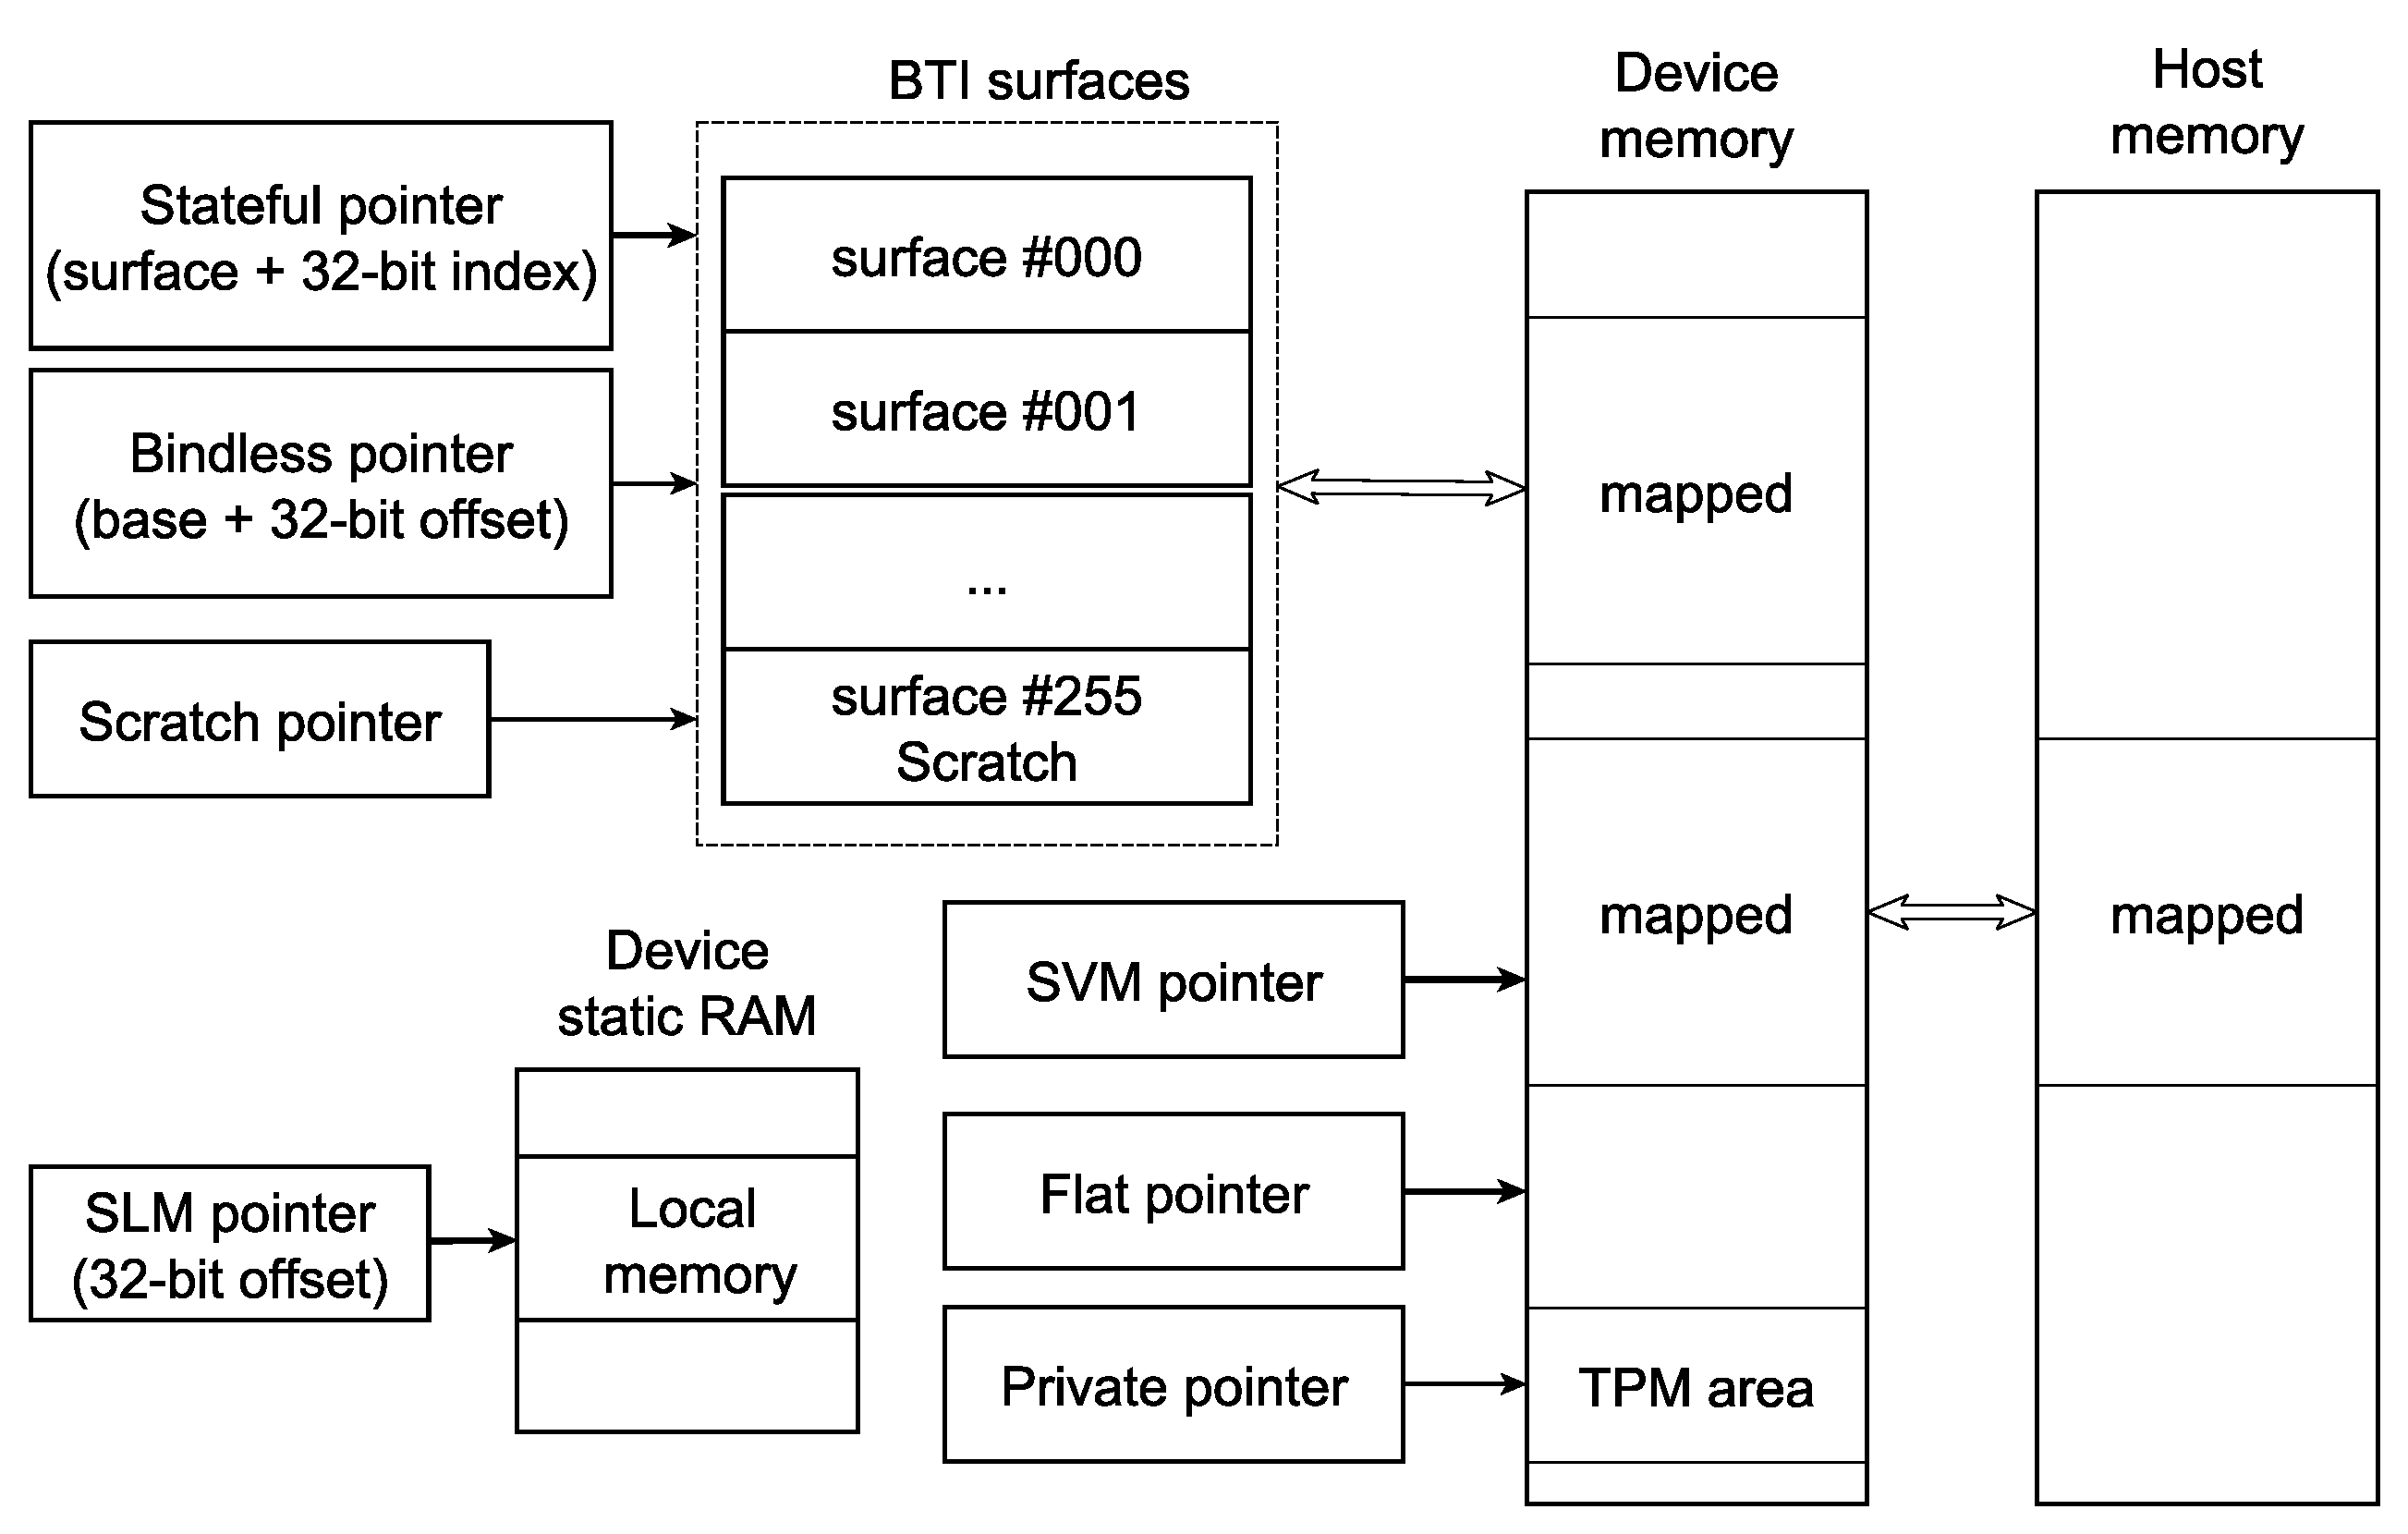
\includegraphics[scale=0.4]{Vladimirov/images/memory-scheme.pdf}
    }
    \caption{Схема физической памяти}\label{fig:memory-scheme}
\end{figure}

На рисунке~\ref{fig:memory-scheme} изображена реалистичная схема физической памяти. Локальная память показана отдельно, так как по сути это кусок L1 кеша на каждом computing unit. Собственно о локальной памяти и можно думать как о своего рода кеше.

Интересно, что само наличие памяти обладающей состоянием является для вычислительных программных интерфейсов в основном прозрачным. Компилятор часто может сделать stateless to stateful преобразование, если он может доказать, что работа ведётся в пределах одного буфера.

Интересной концепцией является приватная память.

\subsection{Векторный характер графических систем команд}\label{subsec:overview/logical/hw}

Все гетерогенные вычисления нужны в основном затем, чтобы максимизировать производительность.
Для этих целей в средней видеокарточке используемой в гетерогенных системах обычно просто нет операционной системы -- её драйвер это драйвер операционной системы хоста.
В связи с эти для таких устройств (это верно и для GPU и для NPU) характерно.

\begin{enumerate}
\item Отсутствие накладных расходов на переключение контекста (нет OS).
\item Сравнительно далёкая и дорогая глобальная память.
\item Часто отсутствие кешей и короткий конвейер.
\end{enumerate}

Всё это мотивирует большие регистровые файлы.

\begin{figure}[ht]
    \centerfloat{
        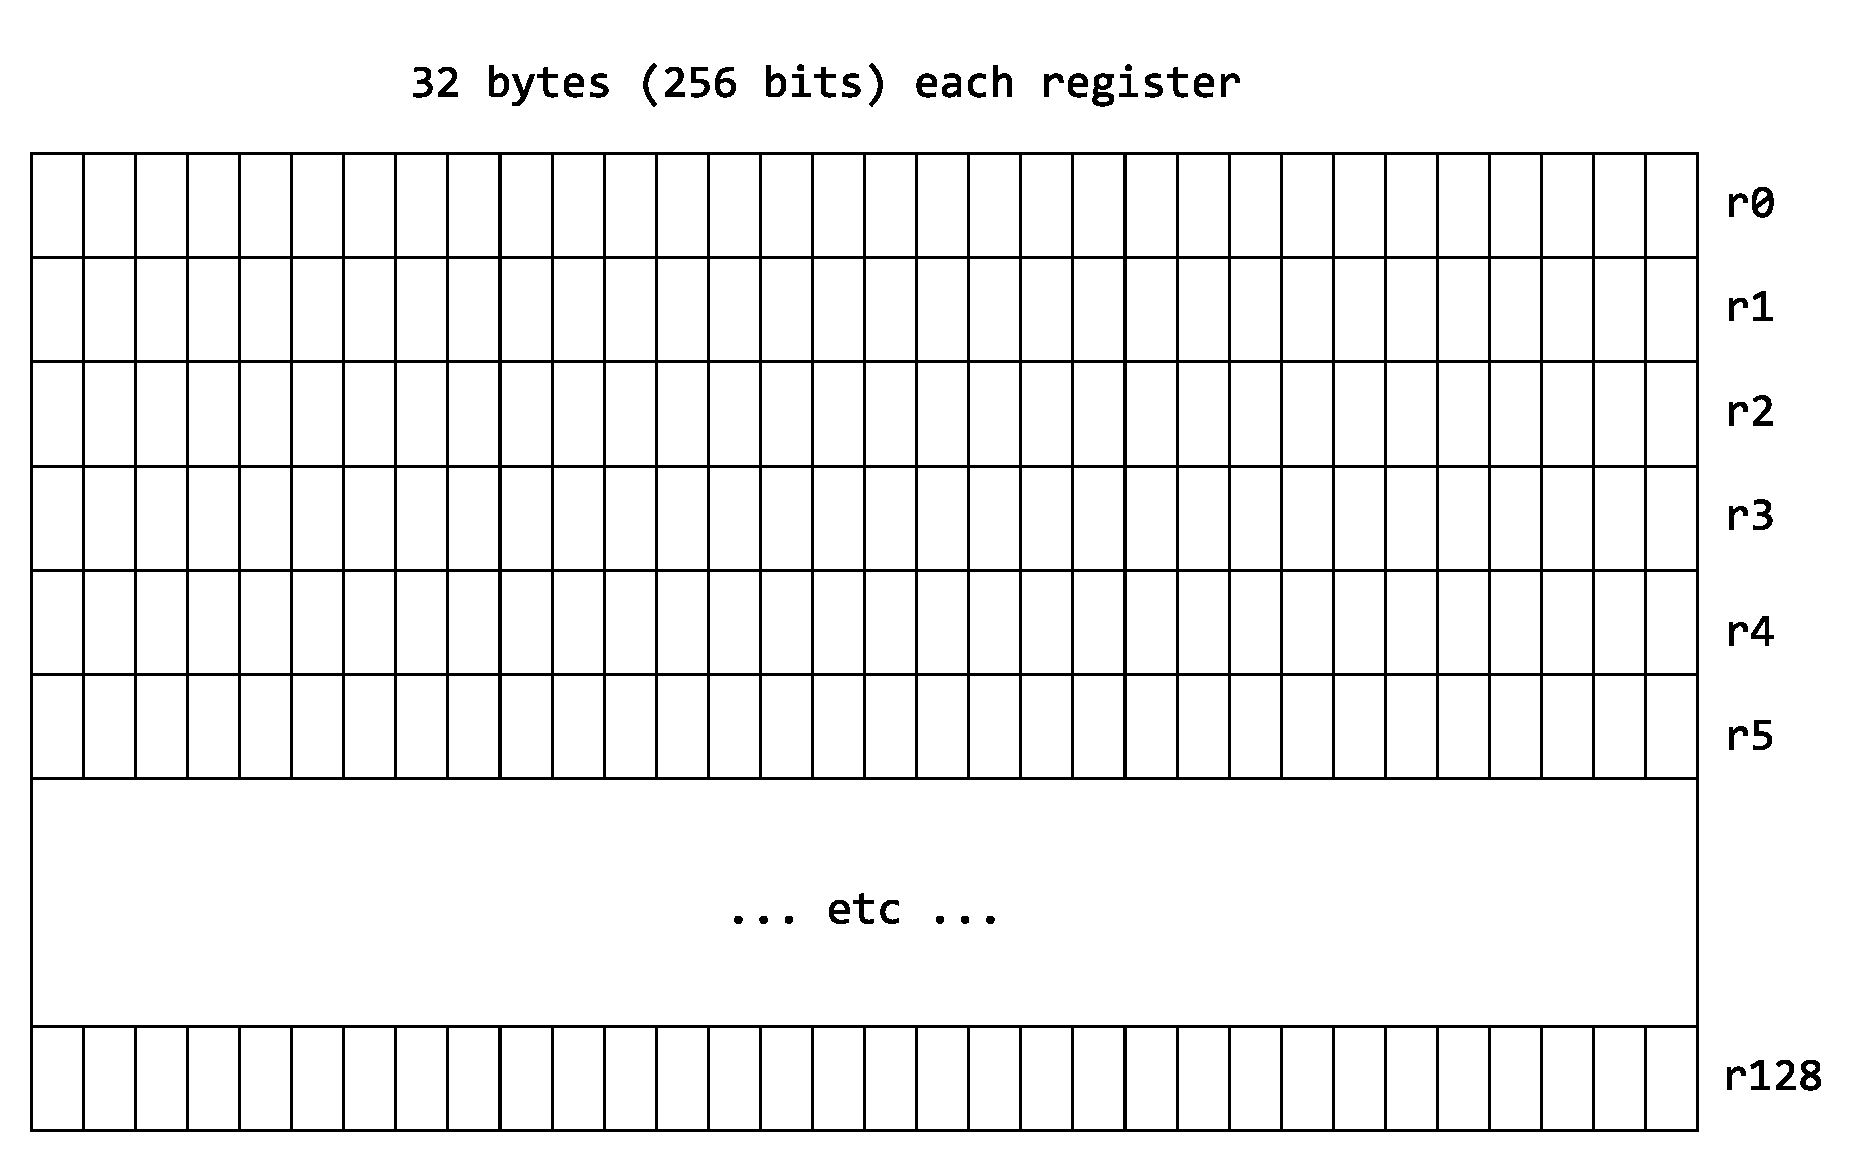
\includegraphics[scale=0.6]{Vladimirov/images/genisa-addressing-base.pdf}
    }
    \caption{Схема регистрового файла}\label{fig:genisa-addressing-base}
\end{figure}

Схема регистрового файла представлена на рисунке~\cref{fig:genisa-addressing-base}

Вовсе не всегда работа с большими регистровыми файлами удобна.

\subsection{Векторный поток управления}\label{subsec:overview/logical/simdcf}

В графических ускорителях многих производителей есть возможность использовать векторный поток управления без сведения его к скалярному случаю. В архитектуре Intel Xe это реализовано через две команды: \texttt{goto} и \texttt{join}. Особенностью команды \texttt{goto} является возможность ее предикатирования. В этом случае исполнение программы произойдет так, что для предикатированных элементов вектора произойдет переход по указанной метке, а для всех остальных элементов произойдет переход на следующую инструкцию. Команда \texttt{join} восстанавливает поток управления.

В аппаратуре подобная модель исполнения реализуется с помощью маски исполнения (\textit{англ. execution mask}). Каждый бит этой маски соответствует элементу вектора. Если бит установлен в 0, то для соответствующего элемента вычисления не производятся, если же бит установлен в 1, то для соответствующего элемента исполнение происходит в обычном режиме. В самом начале программы маска состоит из единиц. Изменения в маске производят инструкции \texttt{goto} и \texttt{join}. Команда \texttt{goto} устанавливает в соответствии с предикатом биты маски в 0, выключая линии вектора, для которых условие не выполняется. Команда \texttt{join} восстанавливает маску до того состояния, в котором она находилась до изменения соответствующим \texttt{goto}.

\begin{ListingEnv}[!h]
    \captiondelim{ } 
    \caption{Пример векторного потока управления}\label{lst:simdcf}
    \begin{Verb}
  ...
  (W)     cmp  (8|M0)  (gt)f0.0  null<1>:d  r2.0<8;8,1>:d -1:w
  (~f0.0) goto (8|M0)            BB_3
  BB_1:
  (W)     add  (8|M0)            r3.0<1>:d  r2.0<8;8,1>:d  1:w
  (f0.0)  goto (8|M0)            BB_5
  BB_2:
          join (8|M0)            BB_3
  BB_3:
          add  (8|M0)            r3.0<1>:d  r2.0<8;8,1>:d -1:w
  BB_4:
          join (8|M0)            BB_5
  BB_5:
  ...
    \end{Verb}
\end{ListingEnv}

На листинге~\cref{lst:oclapi}. пример кода c векторным потоком управления на языке ассемблера для архитектуры графических ускорителей Intel. В данном примере реализовано проверка того, что в регистре r.2.0 лежит значение большее, чем -1, а результат сравнения записан во флаговый регистр f0.0. Далее следует предикатированный регистром f0.0 условный переход: если условие для данной линии исполнения выполняется, то не происходит переход в базовый блок BB\_3, и к данным элементам прибавляется 1, а результат записывается в регистр r3.0. Для других элементов следует переход в базовый блок BB\_3, где из остальных элементов вычитается 1, а результат так же записывается в регистр r3.0.

\begin{figure}[ht]
    \centerfloat{
        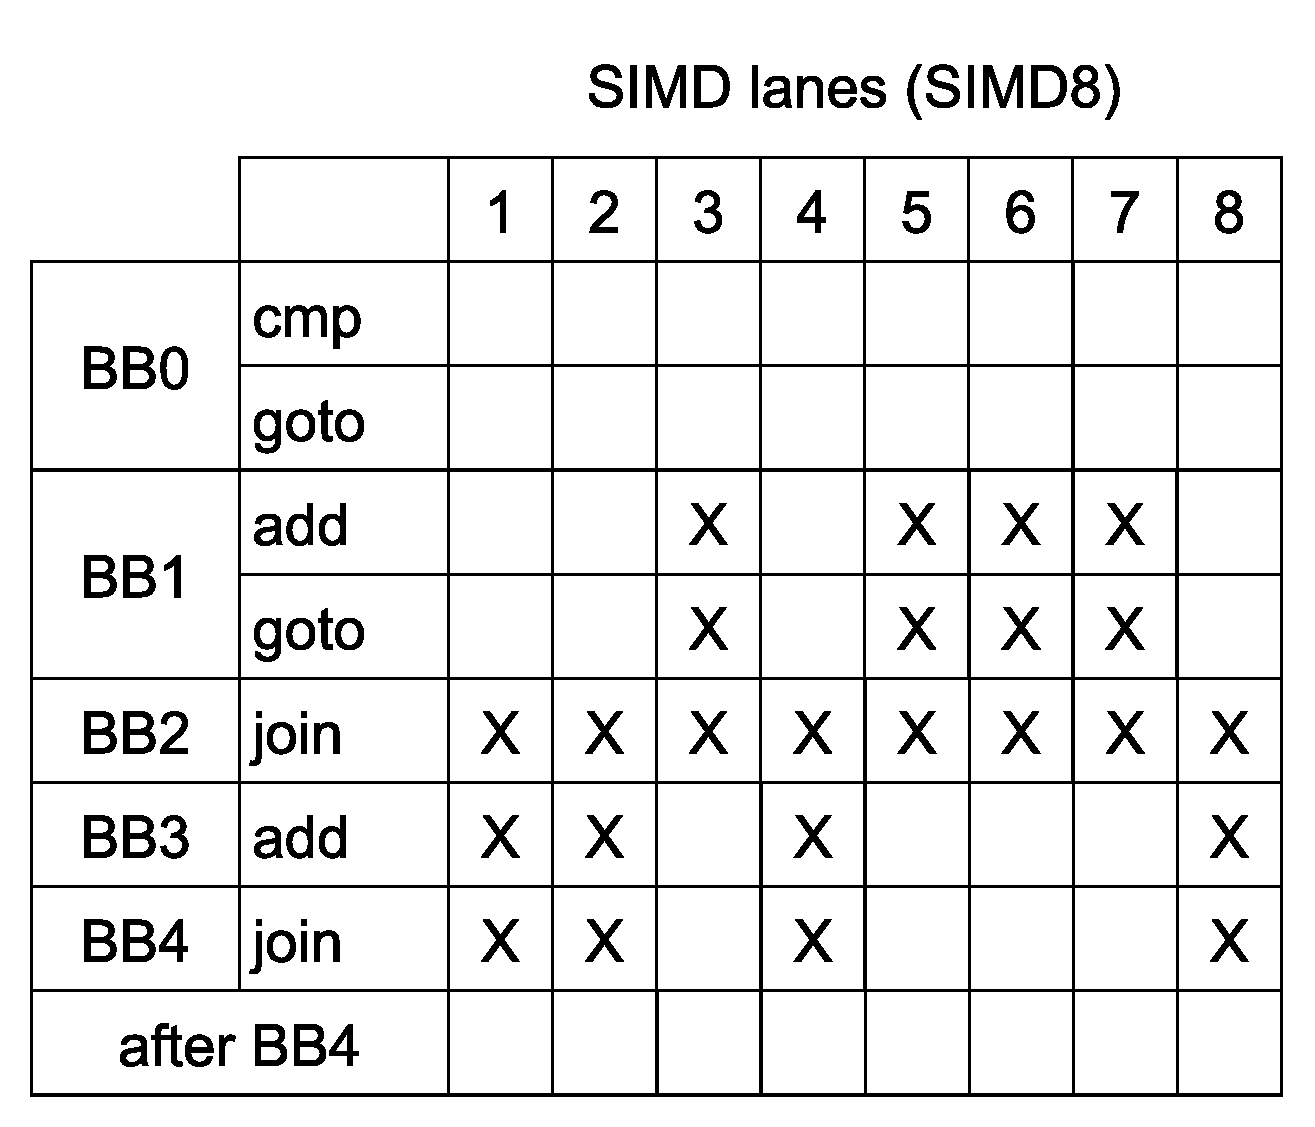
\includegraphics[scale=0.5]{Vladimirov/images/HW-goto-example.pdf}
    }
    \caption{Схема векторного потока управления}\label{fig:HW-goto-example}
\end{figure}

На рисунке~\ref{fig:HW-goto-example} схематично изображено, как будет происходить исполнение данного кода. Цифрами сверху обозначены номера линий исполнения в SIMD АЛУ, зеленым обозначены включенные линии, после исполнения предшествовавшей инструкции, а оранжевым -- выключенные.

\section{Высокоуровневые векторные интерфейсы}\label{sec:overview/vectorapi}

\subsection{ISPC}\label{subsec:overview/vectorapi/ispc}

Тут немного про ISPC

\subsection{DPC++ESIMD}\label{subsec:overview/vectorapi/dpcppesimd}

Тут немного про DPC++ESIMD

\section{Обзор существующих подходов к векторизации}\label{sec:overview/vectorizing}

Большая часть существующих процессоров показывают пиковую производительность благодаря той или иной форме векторизованных инструкций \cite{bialas2015benchmarking}. Это верно и для CPU, например Intel XEON с расширениями AVX и для GPU. Например AMD Graphics Cores Next имеет 64-линейные вектора, а NVIDIA CUDA имеет 32-линейные варпы. Варп \cite{passerat2015warp} это специальный термин для неявного параллелизма обеспечиваемого средствами аппаратного обеспечения. По самой природе таких инструкций, все операции над вектором выполняются одновремено (по крайней мере концептуально). Это ограничивает класс алгоритмов, который может быть эффективно реализован на таких архитектурах. Разумеется цена будет разной при разных подходах.

\subsection{Скалярная ISA и скалярное API}\label{subsec:overview/vectorizing/cuda}

Модель CUDA при реализации высокоуровневой программы делает крайне лёгким написание программы в которой векторный поток управления расходится. Это кстати будет далее характерно и для OpenCL и вообще это верно для любого скалярного API, полагающегося на неявную векторизацию. Она моделирует вычислительную задачу как большое количество потоков исполняющих одну небольшую программу, называемую кернелом или шейдером и для программиста это выглядит как многопоточное параллельное исполнение (SIMT).

\begin{ListingEnv}[!h]
    \captiondelim{ } 
    \caption{Пример кернела на CUDA с замером цикла}\label{lst:cudashader}
    \begin{lstlisting}[language={[ISO]C++}]
__global__ void single_loop(int* limits, float* out) {
  int tid = blockDim.x * blockIdx.x + threadIdx.x;
  int M = limits[threadIdx.x];
  for (int k = 0; k < N_UNROLL; ++k)
    for (int i = 0; i < M; i++)
      sum += EXPR_INNER;
  __syncthreads();
  out[tid] = sum;
}
    \end{lstlisting}
\end{ListingEnv}

Фактически многие руководство CUDA Programming Guide \cite{guide2013cuda} утверждает, что для корректности программист может в целом игнорировать SIMT поведение. Однако серьёзные улучшения производительности могут быть получены если учесть, требует ли код различные потоки внутри варпа расходиться.

На архитектуре NVIDIA потоки группируются в варпы по 32 потока каждый, которые должны исполнять одни и те же инструкции по сути в векторном виде. Из этого следует, что любая инструкция, которая выполняет условный переход, не дающая одного и того же значения в пределах варпа ведёт к неявному расхождению потока управления. В статье про архитектуру Tesla \cite{lindholm2008nvidia} упомянуты механизмы, которыми аппаратура пытается справляться с этой задачей, например стек синхронизации переходов.

\subsection{Векторная ISA и скалярное API}\label{subsec:overview/vectorizing/sycl}

OpenCL, SYCL. Векторизация после основных оптимизаций как часть кодогенерации. Проблемы с векторизацией внешних циклов. Необходимость SIMDX-dispatch, влияние на распределение регистров.

\subsection{Векторное API с ручным управлением регистровым файлом}\label{subsec:overview/vectorizing/cm}

CM. Минимальная роль компилятора. Крайне сложное программирование.

CM (C-for-Metal) -- язык программирования, являющийся расширением С++ и явно реализующий концепцию SIMD. CM является языком с раздельным исходным кодом, то есть компиляция кода хоста и кода устройства происходит раздельно. На данный момент целевыми являются только архитектуры графических ускорителей Intel.

Главной особенностью CM являются новые встроенные типы: \texttt{vector} (вектор), \texttt{vector\_ref} (ссылка на вектор), \texttt{matrix} (матрица) и \texttt{matrix\_ref} (ссылка на матрицу). Каждый из этих типов является шаблонным. Типы \texttt{vector} и \texttt{vector\_ref} имеют два шаблонных параметра: тип элемента и количество элементов. Типы \texttt{matrix} и \texttt{matrix\_ref} имеют три шаблонных
параметра: тип элемента, количество столбцов и количество строк матрицы. Типом элемента может быть любой примитивный целочисленный тип или тип числа с плавающей точкой

\section{Постановка задачи}\label{sec:overview/howtobetter}

В заключение поставим высокоуровневую задачу оптимизирующей компиляции из высокоуровневого векторного программного интерфейса.

Тут продумать постановку. Именно её решает предлагаемая методология в следующей части.

\section{Выводы}\label{sec:overview/outcome}

В первой главе дается общий обзор подходов к компиляции гетерогенных приложений. Рассматривается логическая и физическая модель памяти типичных графических ускорителей. Обосновывается векторный характер регистровых файлов и операций в графических ускорителях. Рассматриваются современные векторные программные интерфейсы, такие как IPSC и DPC++ESIMD, которые становятся актуальны в связи с увеличением сложности задач решаемых современными графическими ускорителями и появления необходимости явно векторизовать вычисления для того, чтобы эффективно класть их на любое устройство, поддерживающее векторизацию (в том числе современные гибридные устройства). 

Проведён подробный анализ существующих подходов к векторизации, который показывает недостаточность существующих методов для эффективного представления векторных программных интерфейсов. Рассмотрены случаи скалряной системы команд с поздней векторизацией или векторной системы команд, с поздней и ранней векторизацией. Видно, что либо векторизация происходит слишком поздно, что не даёт возможности эффективно оптимизировать код на высоком уровне, либо слишком рано, что выключает существующие скалярные оптимизацити.

Недостатки существующих подходов заключаются в их непригодности для отображения высокоуровневых векторных программных интерфейсов на векторную систему команд.

\FloatBarrier